\documentclass[12pt,english,a4paper]{article}
\usepackage[utf8]{inputenc}
\usepackage[T1]{fontenc}
\usepackage{babel,amsmath,amsthm,graphicx,mathtools,textcomp,varioref,amssymb,float,listings}
\usepackage[top=50pt,left=40pt,right=40pt]{geometry}
\usepackage[format=plain,labelfont=bf,up,textfont=it,up]{caption}
\usepackage{titling,wrapfig}
\usepackage{color}
\usepackage{csquotes}
\usepackage{verbatim}
\usepackage{csvsimple}
\usepackage{booktabs}
\usepackage[
backend=biber,
style=alphabetic,
citestyle=authoryear,
sorting=nyt
]{biblatex}

\addbibresource{Data/bibliography.bib}
 
 
\definecolor{codegreen}{rgb}{0,0.6,0}
\definecolor{codegray}{rgb}{0.5,0.5,0.5}
\definecolor{codepurple}{rgb}{0.58,0,0.82}
\definecolor{backcolour}{rgb}{0.95,0.95,0.92}
 
\lstdefinestyle{mystyle}{
    backgroundcolor=\color{backcolour},   
    commentstyle=\color{codegreen},
    keywordstyle=\color{magenta},
    numberstyle=\tiny\color{codegray},
    stringstyle=\color{codepurple},
    basicstyle=\footnotesize,
    breakatwhitespace=false,         
    breaklines=true,                 
    captionpos=b,                    
    keepspaces=true,                 
    numbers=left,                    
    numbersep=5pt,                  
    showspaces=false,                
    showstringspaces=false,
    showtabs=false,                  
    tabsize=2
}
 
\lstset{style=mystyle}


\let\vecarrow\vec
\renewcommand{\vec}[1]{\mathbf{#1}}
\let\oldhat\hat
\renewcommand{\hat}[1]{\oldhat{\mathbf{#1}}}
\def\doubleunderline#1{\underline{\underline{#1}}}
\linespread{1.6}
\renewcommand{\qedsymbol}{$\blacksquare$}

\let\~\tilde

\newcommand{\justdiff}[1]{\frac{\partial}{\partial#1}}
\newcommand{\pdiff}[2]{\frac{\partial #1}{\partial#2}}
\newcommand{\ppdiff}[2]{\frac{\partial^2 #1}{\partial#2^2}}
\newcommand{\proofsquare}{\begin{proof}[] \end{proof}}
\let\f\frac
\DeclareMathOperator{\arccosh}{arcosh}

\DeclarePairedDelimiter\abs{\lvert}{\rvert}%
\DeclarePairedDelimiter\norm{\lVert}{\rVert}%

\makeatletter
\csvset{
  autobooktabularcenter/.style={
    file=#1,
    after head=\csv@pretable\begin{tabular}{*{\csv@columncount}{l}}\csv@tablehead,
    table head=\toprule\csvlinetotablerow\\\midrule,
    late after line=\\\midrule,
    table foot=\\\bottomrule,
    late after last line=\csv@tablefoot\end{tabular}\csv@posttable,
    command=\csvlinetotablerow},
}
\makeatother
\newcommand{\csvautotabularcenter}[2][]{\csvloop{autotabularcenter={#2},#1}}
\newcommand{\csvautobooktabularcenter}[2][]{\csvloop{autobooktabularcenter={#2},#1}}

\tolerance = 5000
\hbadness = \tolerance
\pretolerance = 2000

\title{The Ising Model \\ and some of its thermodynamic properties.}
\author{Jonathan Brakstad Waters\\Øyvind Engebretsen Elgvin\\Henrik Lind Petlund}

\begin{document}

\begin{titlepage}
\vfill
\maketitle
\begin{abstract}

This report studies the thermodynamic properties of the two dimensional Ising Model and demonstrates how a second order phase transition can be described using this binary model. The numerically approximation to the critical temperature of the phase transition is found to be $T_c = 2.885$, which is close to the exact analytical solution in (\cite{LarsOns}). The thermodynamic properties in terms of oscillating energy, configuration of equilibrium, and temperature dependence are shown in various plots.

The report applies the Metropolis algorithm and shows how it can be used to determine whether or not to make a change of a thermodynamic variable (energy). This, combined with the normal probability distribution function, turns out to give satisfying results and simulate the exiting (EXCITING?) phase transition from ferromagnetic to non-magnetic.

\newpage

\end{abstract}
\tableofcontents
\end{titlepage}

\section{Introduction} \label{introduction}

The Ising model is a model that has a large variety of usage. In this report, the model will be used to study phase transitions and thermodynamic properties in magnetic systems. The main goal of the project is to derive the critical temperature for the phase transition from ferromagnetic to paramagnetic. 

The systems at hand are systems of $L\times L$ spins in a two dimensional grid. Each spin may be in either state "up" or "down" denoted with $1$ and $-1$, respectively. The model only focuses on the interaction between the nearest neighbor spins, and the energy between these is given by
\begin{align}
    E = -J \sum_{<kl>}^N s_ks_l 
\end{align}
where $N$ is the number of particles, $s_i=\pm 1$ and $J>0$ is a constant which represents ferromagnetism and the strength of the particle interactions. We assume periodic boundary conditions so that every particle in the lattice has four nearest neighbors. 

Furthermore, the partition function, specific heat capacity, magnetic moment and susceptibility of the system is given by
\begin{equation}
Z=\sum_i e^{-\beta E_i} \label{eq:partition} 
\end{equation}

\begin{equation}
C_V=\frac{1}{k_B T^2}\left(\langle E^2\rangle-\langle E\rangle^2\right)
\end{equation}

\begin{equation}
M=\sum_is_i
\end{equation}

\begin{equation}
\chi= \frac{1}{k_B T}\left(\langle M^2\rangle-\langle M\rangle^2\right)
\end{equation}
as functions of energy and spin, with $\beta =1/k_B T$. These equations are also mentioned in the lecture slides by \cite{LectureIsing} from the course FYS3150.

Initially, we will derive values of a 2x2 case and thereafter, proceed to higher dimensions. In a higher dimension case with $L=20$, the time it takes to reach the most likely state, represented by the number of Monte Carlo cycles, is calculated for two different temperatures with both an ordered and a random initial state. This gives an estimate of the equilibrium time of the system. The energy data from this case is represented by a probability function $P(E)$. 

Next, the systems with $L=40, L=60, L=80$ and $L=100$ are studied as functions of temperature. These calculations are performed to try and simulate phase transitions in the systems. For successfully detected phase transitions, the critical temperature is also extracted and compared to the results yielded by Onsager (1994).

\section{Methods and theory} \label{methods_and_theory}

All data used in this report can be reproduced by running the executable files in the GitHub repository (\cite{GitHub}) and thereafter running the python file \texttt{plot\_data.py}.

\subsection{Monte Carlo method and Metropolis Algorithm}

The heavy calculation in this project is done by using Monte Carlo methods with the \textit{metropolis} algorithm. The steps of our calculation are:

\begin{enumerate}
    \item Initialize an initial state with the energy $E_0$ and magnetic moment $M_0$. This state will have spins in either random directions, or with all spins pointing the same way.
    \item Choose a random spin particle in the lattice, and propose a spin flip. 
    \item Apply the Metropolis Algorithm to decide wether or not to accect the spin flip:
        \begin{enumerate}
            \item Calculate the energy change, $\Delta E=E_1-E_0$, caused by the proposed spin flip. If $\Delta E \le 0$, the spin change is accepted, and we jump to step 4.
            \item If $\Delta E > 0$, calculate the relative probability $w=e^{-\beta \Delta E}$.
            \item For a random number $r \in [0,1]$, if $r \le w$, the new configuration is accepted, otherwise the old configuration is kept.
        \end{enumerate}
    \item Update the expectation values for energy and magnetic moment, and the corresponding heat capacity and susceptibility.
    \item Repeat steps two to four for as longed as desired.
\end{enumerate}

\noindent Steps two to five are called a Monte Carlo Cycle. The number of Monte Carlo cycles, $N$ is determined prior to the calculations. The larger the value for $N$, the better results one should get, as given by the law of large numbers. More details on Monte Carlo methods and the Metropolis Algorithm can be found in the lecture notes for FYS3150 \cite{LectureIsing}. Our implementation of these methods can be found in the program \texttt{Ising\_func\_para.cpp}. 


\subsection{Periodic boundary conditions}
To account for the fact that some of the spins at the boundary of the lattice does not have four nearest neighbours, periodic boundary conditions are introduced. This means that a spin at a boundary i.e. $s_{N,0}$ has a neighbour to the right with the same spin as the particle $s_{0,0}$. In one dimension, this can be expressed by
\begin{align*}
    E_i=-J\sum_{j=1}^{N}s_js_{j+1}
\end{align*}

\noindent as described by \cite{Lec15}. To account for the periodic boundary conditions, we use the function \texttt{Periodic}, found in \texttt{Div\_Functions.cpp}.

For small dimensions, the energy of the system will be significantly affected by whether or not periodic boundary conditions are implemented. As $N \rightarrow \infty$, the boundary becomes insignificant. This is what happens when looking at phase transitions and critical temperatures, where the system has to be described in a larger dimension.

\subsection{Benchmarks}

For the $2x2$ case, the energy, magnetic momentum, specific heat capacity, and the magnetic susceptibility can all be calculated analytically. These analytical values, shown in Table \ref{tab:benchmarks}, are used as benchmarks for the numerically derived values. In our function for the Ising model (As seen in \texttt{Ising\_Func\_Para.cpp} and \texttt{Ising\_Func\_Para\_e.cpp}) we have implemented a test that compares the computed values to the benchmarks. The test is easily callable, and have been used throughout the project to check that the program works after  minor and major changes. 

\subsection{Phase transitions}
In the Ising model, it is interesting to see if it is possible to estimate phase transitions in the systems. These phase transitions can be i.e. liquid/gas (first order) or ferromagnetic/paramagnetic (second order). These transitions are all depending on the parameter $T_C$, called the Curie temperature or the critical temperature. The theory given in the Lecture notes of FYS3150 (\cite{LectureIsing}) can be used to describe some of the values in the Ising model class with a power law behavior as follows
\begin{equation}
    \langle M(T)\rangle\sim (T-T_c)^\beta \propto L^{-\beta/\nu}
\end{equation}
\begin{equation}
    C_V(T)\sim (T-T_c)^{-\gamma} \propto L^{-\alpha/\nu}
\end{equation}
\begin{equation}
    \chi(T)\sim (T-T_c)^\alpha \propto L^{-\gamma/\nu}
\end{equation}
where $\beta = 1/8$ is the so called critical exponent, $\alpha = 0$ and $\gamma = 7/4$. The value of $\nu$ is defined by the correlation length which has a divergent behavior when approaching $T_c$
\begin{equation}
      \xi(T) \propto L \sim \left|T_C-T\right|^{-\nu},
  \label{eq:xi}
\end{equation}

\noindent The lattice sizes in this report are always finite, and therefore $\chi$ will be proportional to this lattice size as seen in the equations above. Using finite size scaling relations, it is possible to relate the results and behaviors in the finite lattices with the ones from the infinite case. This results in a scaling of the critical temperature given by

\begin{equation}
    T_C(L)-T_C(L=\infty) = aL^{-1/\nu} \label{eq:tc}
\end{equation}
with $\nu = 1$. The exact result for $T_c(L=\infty)$ is found in (\cite{LarsOns}), and is given as the dimensionless value
\begin{align*}
    kT_c/J=\frac{2}{ln(1+\sqrt{2})}=2.269
\end{align*}
If a phase transition is observed in a finite system, the critical temperature, $T_{c}(L_i)$, is possible to derive. The value of $T_{c}(L=\infty)$ can be derived if one has two temperatures or more from finite systems by using Equation \eqref{eq:tc}. This would result in a couple of equations with two unknown variables; $T_c(L=\infty)$ and $a$, given by
\begin{align*}
    \begin{cases}
        T_c(L=\infty)=T_c(L_1)-aL_1^{-1/\nu}\\
        T_c(L=\infty)=T_c(L_2)-aL_2^{-1/\nu}
    \end{cases}
\end{align*}
\noindent By eliminating $a$, we get the following expression for the critical temperature of an infinite lattice: 
\begin{equation}
    T_c(L=\infty) = \frac{L_2 T_c(L_2) - L_1 T_c(L_1)}{L_2-L_1}
    \label{eq:Tc_inf}
\end{equation}

Alternatively, one could use \texttt{NumPy}'s \texttt{polyfit}, do a linear regression for several experimental temperatures and find an approximation to the curve
\begin{align*}
        T_C(L) = T_C(L=\infty)+aL^{-1/\nu}
\end{align*}
where $T_c(L=0)$ gives the critical temperature of the infinite system. 

We have tried both methods. For the regression, we used four lattice sizes, $L \in [40,60,80,100]$. For the use of equation (\ref{eq:Tc_inf}), we have set $L_1 = 40$ and $L_2 = 100$. To find $T_c$ for each lattice, we have plotted the heat capacity $C_V$ as function of temperature. The critical temperature for each lattice is read as the one corresponding to the maximum value of $C_V$. 

It turns out that the use of equation (\ref{eq:Tc_inf} yields the better results when comparing with \cite{LarsOns}, and so those are the results we will present.

\section{Results} \label{results}

\subsection{The 2x2 Case}

Table \ref{tab:configurations} lists the different possible spin configurations with their respective degeneracy, energy and magnetization in the 2x2 lattice, whereas Table \ref{tab:benchmarks} displays the analytic and experimental values of interest in the 2x2 lattice.

\begin{table}[H]
    \centerline{\csvautobooktabularcenter{Data/E_M_Configurations.csv}}
    \caption{List of the different possible spin configurations with their respective degeneracy, energy and magnetization in the 2x2 case.}
    \label{tab:configurations}
\end{table}

\begin{table}[H]
    \centerline{\csvautobooktabular{Data/Benchmarks.csv}}
    \caption{List of analytical and experimental values for the $2x2$ lattice with the absolute relative deviation. All values are scaled by the number of spin ($L^2$).}
    \label{tab:benchmarks}
\end{table}

\newpage

\subsection{The most likely state}

Figure \ref{fig:E_equiv} and Figure \ref{fig:M_equiv} gives a graphical presentation of the time ($\#$ of MC-cycles) it takes for different systems to reach equilibrium. Depending on the ordering of the initial state and the temperature of the different systems; an estimate of the equilibrium time can be made. Figure \ref{fig:acc_conf} gives the number of accepted configurations as function of MC-cycles.

\begin{figure}[H]
    \centering
    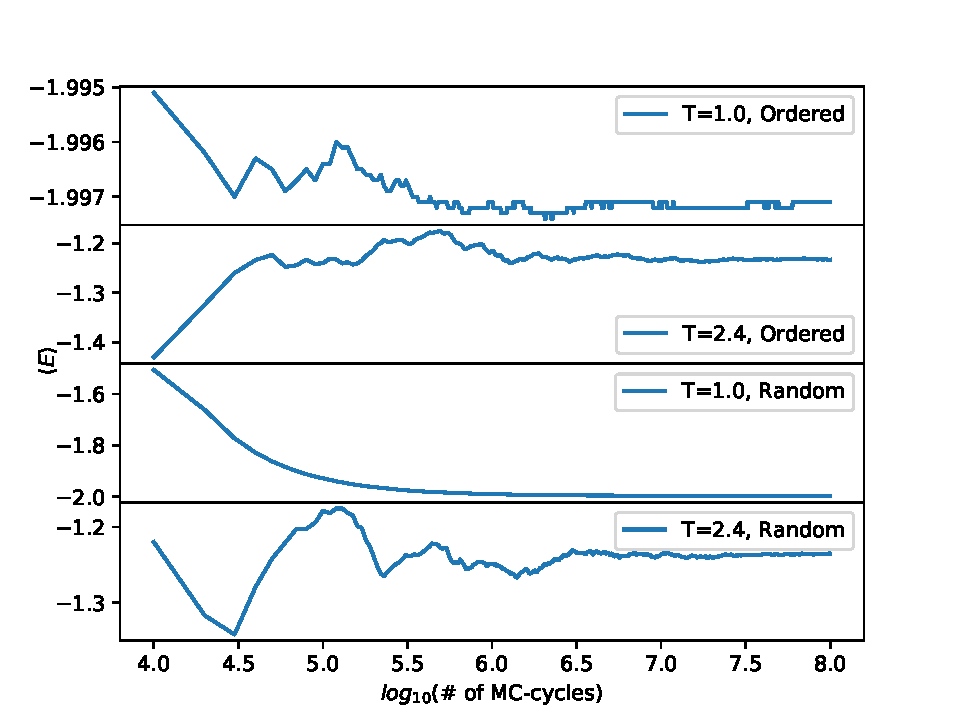
\includegraphics[scale=0.7]{Figures/Most_Likely_State_E_mean_L_20.pdf}
    \caption{The mean energy for temperatures $T=[1.0,2.4]$ for both an ordered and random initial state as function of MC-cycles (time), L = 20. The x-axis is logarithmically scaled and there are $10^4$ MC-cycles between each data point.}
    \label{fig:E_equiv}
\end{figure}
\begin{figure}[H]
    \centering
    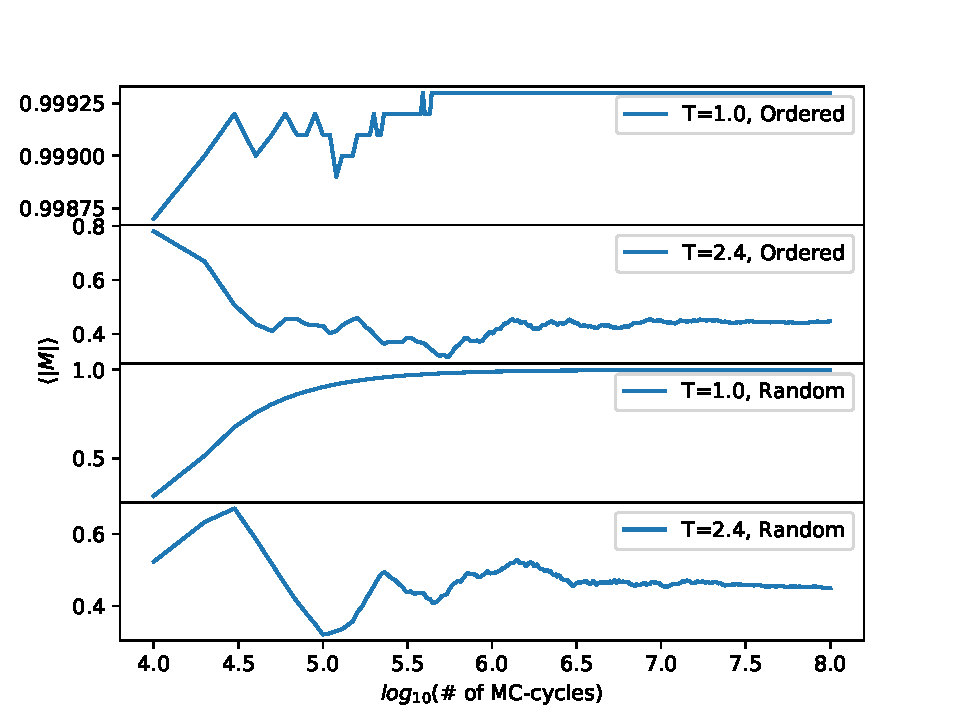
\includegraphics[scale=0.7]{Figures/Most_Likely_State_M_abs_L_20.pdf}
    \caption{The mean absolute magnetization for temperatures $T=[1.0,2.4]$ for both an ordered and random initial state as function of MC-cycles (time), L = 20. The x-axis is logarithmically scaled and there are $10^4$ MC-cycles between each data point.}
    \label{fig:M_equiv}
\end{figure}
\begin{figure}[H]
    \centering
    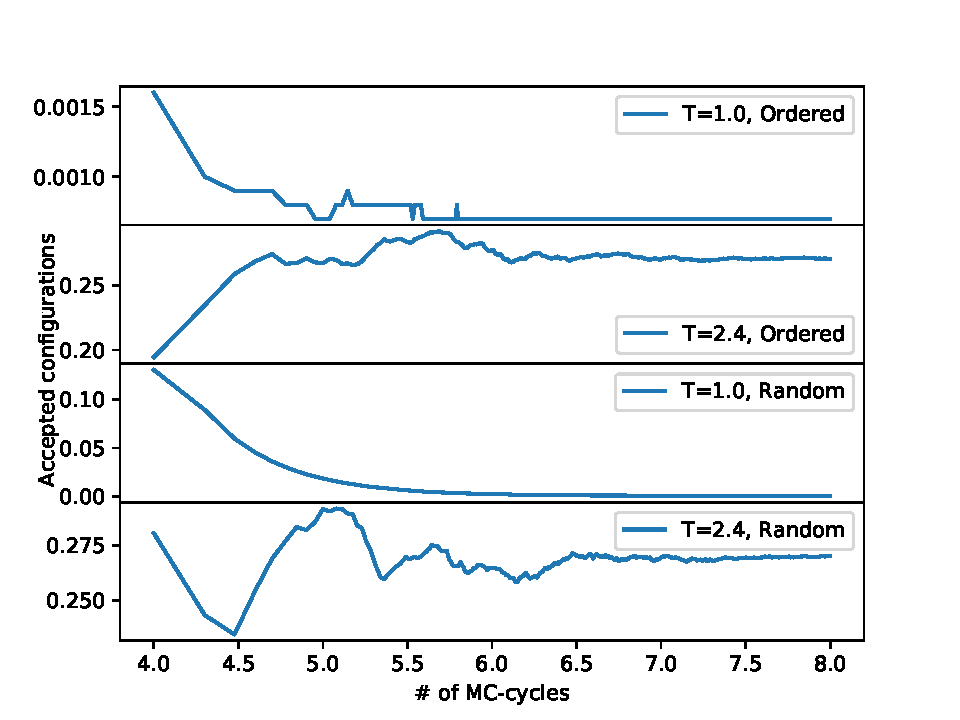
\includegraphics[scale=0.7]{Figures/Number_of_Accepted_Configs_L_20.pdf}
    \caption{Number of accepted configurations per MC-cycle for temperatures $T=[1.0,2.4]$, for both an ordered and a random initial state as function of MC-cycles (time), L = 20. The x-axis is logarithmically scaled there are $10^4$ MC-cycles between each data point.}
    \label{fig:acc_conf}
\end{figure}

\subsection{The Probability Distribution}
Figure \ref{fig:probability} displays the probability distribution of energies for temperatures $T=1.0$ and $T=2.4$. For $T=2.4$, the program \texttt{plot\_data.py} calculates (by integration) that $67.93\%$ of the data points are withing the first order standard deviation.
\begin{figure}[H]
    \centering
    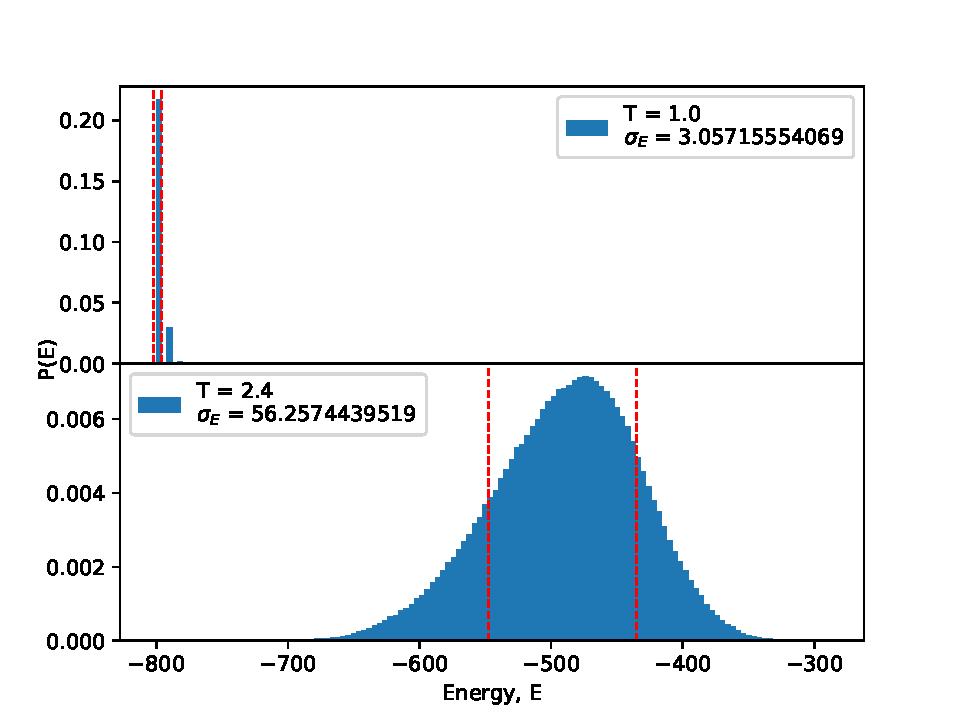
\includegraphics[scale=0.7]{Figures/Probability_Distribution_N_1000000000_L_20.pdf}
    \caption{Probability distribution of the energy, $E$, in a lattice of size L = 20 for temperatures $T = [1.0,2.4]$. The data comes from $10^7$ energies that are collected after equilibrium has been reached (here; $10^8$ MC-cycles). The red dashed lines shows the first order standard deviation, $\sigma_E$, from the mean energy.}
    \label{fig:probability}
\end{figure}

\subsection{Phase transitions and the critical temperature, $T_c$}

Figure \ref{fig:E_of_T}-\ref{fig:X_of_T} in section \ref{appendix} shows $\langle E\rangle$, $\langle |M|\rangle$, $C_v$ and $\chi_{abs}$ as function of temperature. By the use of Equation \eqref{eq:tc}, and the maxima of the $C_v$ curve, the critical temperature of the infinite lattice is derived numerically in \texttt{plot\_data.py}. Table \ref{tab:critical} compares this to the one derived in \cite{LarsOns}. 

\begin{table}[H]
    \centerline{\csvautobooktabular{Data/critical.csv}}
    \caption{Experimentally derived critical temperature, $T_c(L=\infty)$, compared to the exact temperature by \cite{LarsOns}.}
    \label{tab:critical}
\end{table}

\section{Discussion} \label{discussion}

\subsection{The 2x2 Case}
As seen by table \ref{tab:benchmarks}, the values computed by our program are quite accurate with respect to the analytical values. One may see that the relative deviation from the analytical values are largest in terms of $\langle C_v \rangle$ and $\chi _abs$. This is not very strange, noting that those values are calculated using $\langle E \rangle$ and $\langle M \rangle$. It is only natural that using erroneous values to compute other values, yields less precision in the final result.   However, one would maybe expect $\chi$ to be deviating by a similar amount - it is not easy to say why this is not the case. 

It seems clear by the benchmark comparison that our program runs properly and yields correct results for the 2x2 case. This gives reason to believe that our results for higher values of $L$ are also plausible. 

\subsection{The most likely state}
In figures \ref{fig:E_equiv} and \ref{fig:M_equiv}, we have plotted the time evolution (given by the number of Monte Carlo Cycles) of the energy and absolute magnetic moment of the system. For low temperatures ($T = 1$), the system should be in the ground state, with ordered spins and low energy. We see that this is the case - after a number of MC cycles, the energy stabilizes at approximately $-1.997$ pr spin. This seems to take about the same amount of time ($\sim 10^7$ MC-cycles) regardless of what initial state the system is in - ordered or random. 

For higher temperatures ($T=2.4$), the equilibrium state has considerably higher energy, somewhere around $-1.2$ pr spin. However, for the magnetic moment, we see the opposite trend - for low temperatures, the mean magnetic moment pr. spin stabilizes at about $1$, whilst for higher temperatures, it stabilizes at about $0.5$. This is easily explained if we note that for the ground state, all the spins should point in the same direction. Hence, the total magnetic moment pr. spin is 
\begin{align*}
    M = \frac{1 \cdot L^2}{L^2} = 1
\end{align*}
Note that if we plotted $\langle M \rangle$ instead of $\langle |M| \rangle$, this value could just as well be $-1$, depending on the initial configuration.

For higher temperatures, the spins are configured in a more random manner, and hence the magnetic moment pr. spin is no longer equal to one. In fact, for high temperatures, one would expect the magnetic moment to go to zero, as seen for $L=100$ in Figure \ref{fig:M_of_T}. The 20x20 case is probably not large enough to properly illustrate this development. 

In Figure \ref{fig:acc_conf}, the number of accepted configurations pr Monte Carlo cycle is plotted. One can see that these plots coincides well with the earlier discussed plots for the energy and the magnetic moment. When starting off in the ground state at some low temperature, the likelihood of moving into a higher energy state is very low. As a result, one would expect that few of the proposed spin flips are accepted. This is also what we see - when the system has reached equilibrium, the number of accepted flips is basically zero. For higher temperatures, the likelihood of proposing a state with lower or higher energy than the equilibrium state is much higher - hence, we see that the number of accepted flips pr. cycle is approximately 0.27.

This increase in accepted flips per cycle will in turn reveal a larger fluctuation in energy as time passes. Looking at the axis of the energy plots - it is easily observed that at higher temperatures, the energy fluctuations at equilibrium are much larger. The next section gives a deeper explanation of this.

\subsection{Probability Distribution}
The fluctuations discussed in the above subsection may now be addressed further. The plots showing the equilibrium time are great when estimating there to begin precise calculations. However, they do not give a good indication of the values of the possible energy states and how likely they are to be possessed by the system - in comes the probability distribution.

In Figure \ref{fig:probability} in Section \ref{results}, the experimental probability distribution for the low temperature case and the high temperature case is given. A first glance at the high temperature distribution gives a good impression of a normal distribution. This correlates well with the fact that the random number generator used in the metropolis algorithm is in fact based on the normal distribution.

As for the low temperature case, there are just three different energies in the distribution (may be more, but only observing with the naked eye). The largest column is the one for the ground state energy, and reflects the fact that the system at low temperatures prefers a lower energy than the system at high temperatures. This column thereby represents the most likely energy state at $T=1.0$, and is in fact also the lowest possible energy a system of this kind may have. Because of this it is obvious why the distribution isn't broadening towards higher (and lower) energies, such as it does in the high temperature case. This broadening reflects the possibility for the system to oscillate in energy at higher temperatures, even though equilibrium has been reached.

It is interesting to compare the standard deviation, $\sigma_E$, (and therefore also the variance, $\sigma_E^2$) of the two different temperature cases (red dotted lines in Figure \ref{fig:probability}). At $T=1$, the STD is low (compared to $T=2.4$), which is an intuitive and direct result of the fact that the energy is bound to low values. As for $T=2.4$, the STD increases a lot more and looks more like the first order STD of the normal distribution. An ideal normal distribution curve has $\sim 68\%$ of its data points within the first order STD. From Section \ref{results}, the probability distribution at $T=2.4$ has $67.93\%$ of its data points withing the first order STD - which coincides well with that of the normal distribution!

\subsection{Phase transitions and the critical temperature, $T_c$}

The critical temperature is where the system turns from magnetic to non-magnetic, or from ferromagnetic to paramagnetic, but these temperatures are scaled and, therefore, not to be taken as kelvin. As seen in Table \ref{eq:tc}, the experimental critical temperature is calculated to be 2.2885, with a relative deviation of $\sim 0.2\%$ from the exact value calculated in (\cite{LarsOns}). Our calculation was done as described in section \ref{methods_and_theory}, using our maximum values for $Cv$ to approximate the critical temperature for an infinitely large lattice. It could well be that our result would have been closer to the exact value if our lattice sizes were larger, or we calculated with more Monte Carlo Cycles or for more temperatures on our interval. However, that would be time consuming, and we have tried to strike a good compromise between precision and runtime. 

In figure 6, we see that the magnetization phase quickly turns non-magnetic around the critical temperature as the temperature rises, which makes sense since the entropy of the system rises with the rise of temperature, and a magnetic phase is then hard to sustain. 

Figure \ref{fig:X_of_T}, clearly shows how the susceptibility peaks around the critical temperature, and that the larger the system is the higher the peak is. 

HER ER DET BARE Å FYLLE INN ELLER EDITERE OVER HER GUTTER.. 

\section{Conclusion} \label{conclusion}

In this project, we have used Monte Carlo Methods with the Metropolis Algorithm to model a ferromagnetic system with the use of the Ising Model. The goal of this project was to find a critical temperature for the phase transition from magnetic to non-magnetic in the binary system.

The basic idea of the model was to construct an $L \times L$ lattice with spins pointing either up or down. Then we proposed $N$ number of spin flips, and either accept or reject these based on a sample rule. As more and more spin flips where proposed, the system developed towards an equilibrium state, and allowed us to calculate expectation values for the energy and the magnetic moment. In turn, these values made it easy to calculate the heat capacity and susceptibility of the system as the variances of Energy and magnetic moment respectively. 

We have analyzed the above mentioned values for a number of different temperatures. From equations for finite lattice scaling we found an estimate for the critical temperature for the phase transition. The critical temperature was found to be $Tc = 2.2885$.


\section{Appendix} \label{appendix}

\subsection{Calculating the benchmarks}

Finding the analytical values, we start by calculating the energies for the configurations of all possible spins. The number of configurations in the $2x2$ case is  $2^4 = 16$, in total. The energies are given by summing the interaction between the four neighbors
\begin{align*}
    E = -J \sum_{<kl>}^N s_ks_l 
\end{align*}
where an interaction is one of the four possible:
\begin{align*}
    E_{\uparrow \uparrow} = E_{\downarrow \downarrow} = -2J, 
\end{align*}
\begin{align*}
    E_{\uparrow \downarrow} = E_{\downarrow \uparrow} = 2J
\end{align*}
The $2x2$ case can then be divided in degeneracy of energies by how many spin up there is
\begin{align*}
    E_{\text{4 spin}\uparrow} = (-2J) + (-2J) + (-2J) + (-2J) = -8J \text{ with degeneracy = 1}
\end{align*}
\begin{align*}
    E_{\text{3 spin}\uparrow} = 2J + (-2J) + 2J + (-2J) = 0 \text{ with degeneracy = 4}
\end{align*}
\begin{align*}
    E_{\text{2 spin}\uparrow} = (-2J) + 2J + (-2J) + 2J = 0 \text{ with degeneracy = 4}
\end{align*}
\begin{align*}
    E_{\text{2 spin}\uparrow} = 2J + 2J + 2J + 2J = 8J \text{ with degeneracy = 2}
\end{align*}
\begin{align*}
    E_{\text{1 spin}\uparrow} = 2J + 2J + (-2J) + (-2J) = 0 \text{ with degeneracy = 4}
\end{align*}
\begin{align*}
    E_{\text{0 spin}\uparrow} = (-2J) + (-2J) + (-2J) + (-2J) = -8J \text{ with degeneracy = 1}
\end{align*}
with the associated magnetic moment, $M$, calculated for each spin configuration as
\begin{align*}
    M_{i}=\sum_{j=1}^{N} s_{j}
\end{align*}
as shown table 1.

With these energies, degeneracies, magnetization, and periodic boundary conditions we can calculate the analytical benchmark expressions, starting with the participation function, which is calculated as
\begin{align*}
    Z = \sum_{i=1}^{2^n} e^{-\beta E_i}
      = 2e^{\beta 8J} + 2e^{-\beta 8J} + 12
      = 4cosh(\beta 8J) + 12
\end{align*}
The expectation value for the energy
\begin{align*}
    <E> \hspace{0.2cm} 
        = \sum_{i=1}^{2^n} E_iP_i(T) 
        = \frac{1}{Z} \sum_{i=1}^{16} E_ie^{-\beta E_i}
        = - \frac{\delta ln(Z(T))}{\delta \beta}
        = -\frac{32sinh(\beta 8J)}{4cosh(\beta 8J) + 12}
\end{align*}
and the expression for the expectation value for the energy squared
\begin{align*}
    <E^2> \hspace{0.2cm} 
          = \sum_{i=1}^{2^n} E_i^2P_i(T) 
          = \frac{1}{Z} \sum_{i=1}^{16} E_i^2e^{-\beta E_i}
          = \frac{128J^2e^{\beta 8J} + 128J^2e^{-\beta 8J}}
                 {4cosh(\beta 8J) + 12}
          = \frac{64J^2cosh(\beta 8J)}{cosh(\beta 8J) + 3}
\end{align*}
The specific heat capacity take the expression
\begin{align*}
    C_v = \frac{\sigma_E^2}{k_BT^2} 
\end{align*}
where the variance, $\sigma_E^2$, is
\begin{align*}
    \sigma_E^2 = \hspace{0.2cm} <E^2> - <E>^2 \hspace{0.2cm}
               = \frac{64J^2cosh(\beta 8J)}{cosh(\beta 8J) + 3}
               - \bigg(-\frac{32sinh(\beta 8J)}{4cosh(\beta 8J) + 12}\bigg)^2
\end{align*}
Similarly, the analytic expressions of the magnetic moment are calculated as
\begin{align*}
    <M> \hspace{0.2cm} 
        = \sum_{i=1}^{2^n} M_iP_i(\beta) 
        = \frac{1}{Z} \sum_{i=1}^{16} M_ie^{-\beta E_i} = 0 
\end{align*}
and the mean absolute value of the magnetic moment is given by 
\begin{align*}
    <|M|> \hspace{0.2cm} 
          = \sum_{i=1}^{2^n} |M_i^2P_i(\beta)| 
          = \frac{1}{Z} \sum_{i=1}^{16} |M_i^2e^{-\beta E_i}|
          = \frac{8e^{\beta 8J} + 16}{4cosh(\beta 8J) + 12}
          = \frac{2e^{\beta 8J} + 4}{cosh(\beta 8J) + 3}
\end{align*}
Further
\begin{align*}
    <M^2> \hspace{0.2cm} 
          = \sum_{i=1}^{2^n} M_i^2P_i(\beta) 
          = \frac{1}{Z} \sum_{i=1}^{16} M_i^2e^{-\beta E_i}
          = \frac{32e^{\beta 8J} + 32}
                 {4cosh(\beta 8J) + 12}
          = \frac{8e^{\beta 8J} + 8}{cosh(\beta 8J) + 3}
\end{align*}
may give the magnetic variance as
\begin{align*}
    \sigma_M^2 = \hspace{0.2cm} <M^2> - <M>^2 \hspace{0.2cm}
               = \hspace{0.2cm} <M^2> - \hspace{0.2cm} 0
               = \frac{8e^{\beta 8J} + 8}{cosh(\beta 8J) + 3}
\end{align*}
and the absolute magnetic variance is as
\begin{align*}
    \sigma^2_{M,abs} = <M^2> - <|M|>^2 = \frac{8e^{\beta 8J} + 8}{cosh(\beta 8J) + 3}+\frac{2e^{\beta 8J} + 4}{cosh(\beta 8J) + 3}= \frac{10e^{\beta 8J} + 12}{cosh(\beta 8J) + 3}
\end{align*}
Such that the analytical value of the susceptibility and the absolute susceptibility can be calculated by
\begin{align*}
    \chi = \frac{\sigma_M^2}{k_BT}
\end{align*}

\subsection{Figures}

Figure \ref{fig:E_of_T}-\ref{fig:X_of_T} shows $\langle E\rangle$, $\langle |M|\rangle$, $C_v$ and $\chi_{abs}$ as function of temperature. All figures can be reproduced by running \texttt{phase\_exe} followed by \texttt{plot\_data.py}.

\begin{figure}[H]
    \centering
    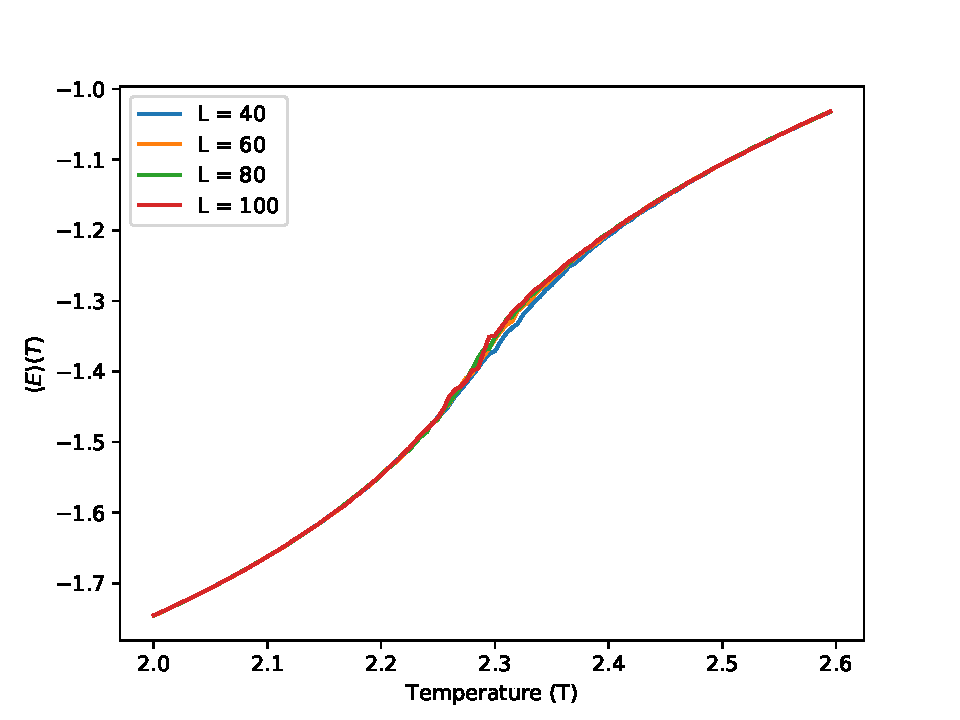
\includegraphics[scale=0.7]{Figures/E_of_T_N_1000000000.pdf}
    \caption{The mean energy as function of temperature, T, for lattice sizes 40, 60, 80 and 100.}
    \label{fig:E_of_T}
\end{figure}
\begin{figure}[H]
    \centering
    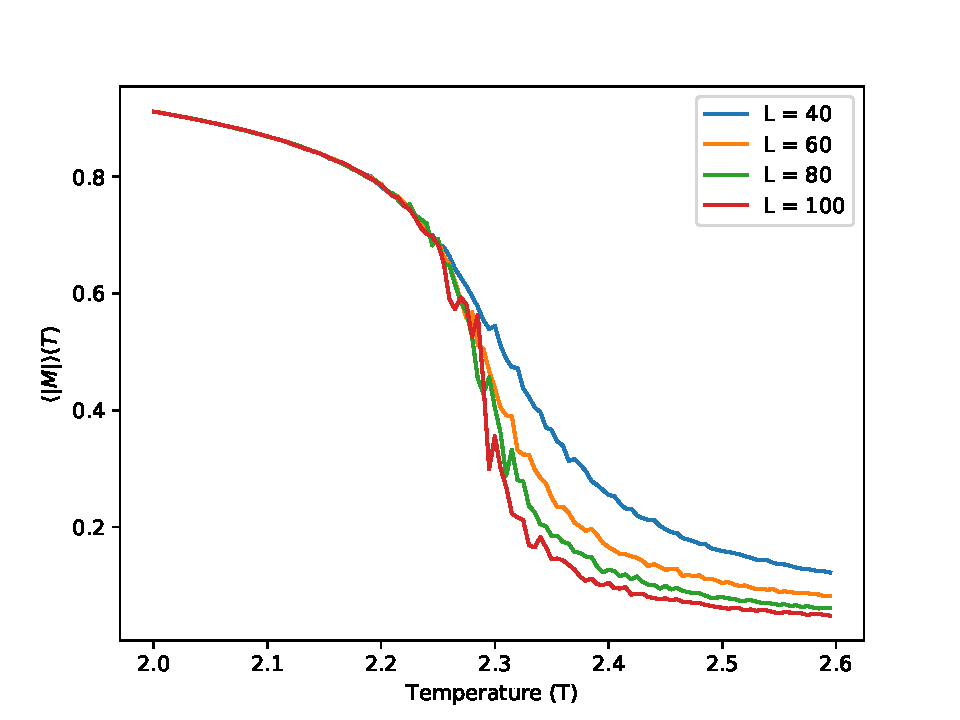
\includegraphics[scale=0.7]{Figures/M_of_T_N_1000000000.pdf}
    \caption{The mean absolute magnetization as function of temperature, T, for lattice sizes 40, 60, 80 and 100.}
    \label{fig:M_of_T}
\end{figure}
\begin{figure}[H]
    \centering
    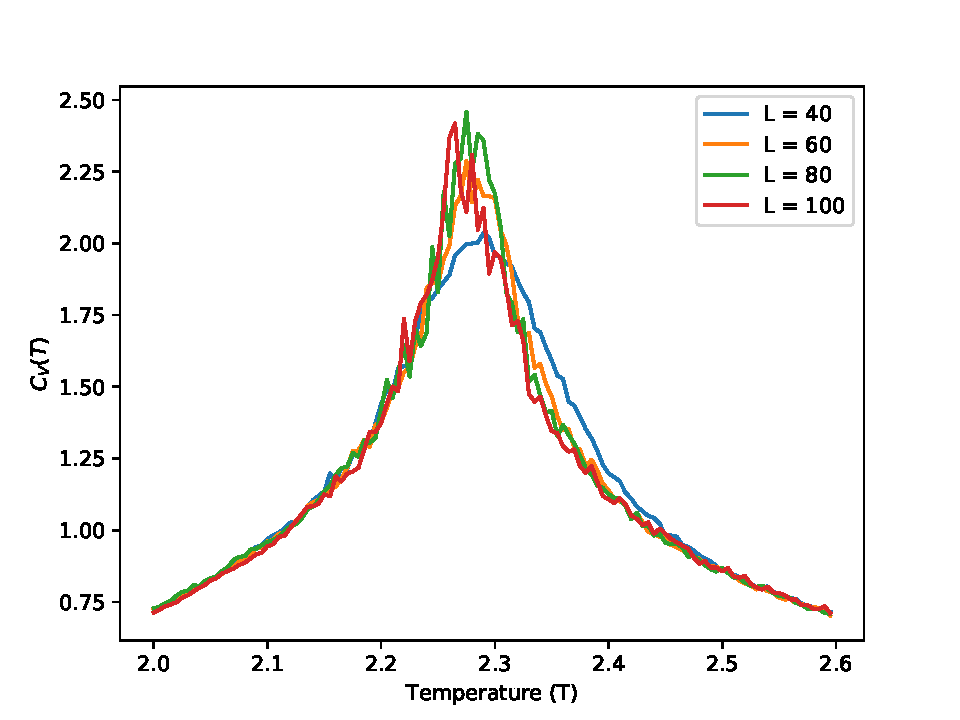
\includegraphics[scale=0.7]{Figures/Cv_of_T_N_1000000000.pdf}
    \caption{The heat capacity as function of temperature, T, for lattice sizes 40, 60, 80 and 100.}
    \label{fig:Cv_of_T}
\end{figure}
\begin{figure}[H]
    \centering
    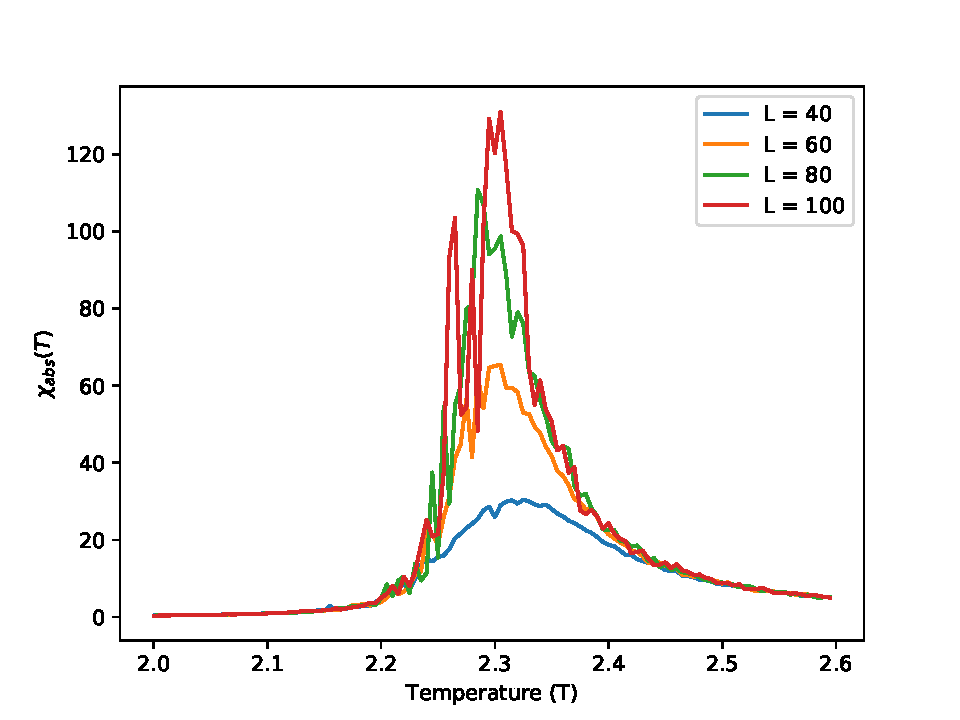
\includegraphics[scale=0.7]{Figures/X_of_T_N_1000000000.pdf}
    \caption{The susceptibility as function of temperature, T, for lattice sizes 40, 60, 80 and 100.}
    \label{fig:X_of_T}
\end{figure}


\printbibliography


\end{document}
